%% Преамбула TeX-файла

% 1. Стиль и язык
\documentclass[utf8x, 14pt]{G7-32} % Стиль (по умолчанию будет 14pt)

% Остальные стандартные настройки убраны в preamble.inc.tex.
\sloppy

% Настройки стиля ГОСТ 7-32
% Для начала определяем, хотим мы или нет, чтобы рисунки и таблицы нумеровались в пределах раздела, или нам нужна сквозная нумерация.
\EqInChapter % формулы будут нумероваться в пределах раздела
\TableInChapter % таблицы будут нумероваться в пределах раздела
\PicInChapter % рисунки будут нумероваться в пределах раздела
\usepackage{slashbox}

% Добавляем гипертекстовое оглавление в PDF
\usepackage[
bookmarks=true, colorlinks=true, unicode=true,
urlcolor=black,linkcolor=black, anchorcolor=black,
citecolor=black, menucolor=black, filecolor=black,
]{hyperref}

% Изменение начертания шрифта --- после чего выглядит таймсоподобно.
% apt-get install scalable-cyrfonts-tex

\IfFileExists{cyrtimes.sty}
    {
        \usepackage{cyrtimespatched}
    }
    {
        % А если Times нету, то будет CM...
    }

\usepackage{graphicx}   % Пакет для включения рисунков

% С такими оно полями оно работает по-умолчанию:
% \RequirePackage[left=20mm,right=10mm,top=20mm,bottom=20mm,headsep=0pt]{geometry}

\geometry{right=20mm}
\geometry{left=30mm}


% Пакет Tikz
\usepackage{tikz}
\usetikzlibrary{arrows,positioning,shadows}
\usepackage{pgfplots}

% Произвольная нумерация списков.
\usepackage{enumerate}

% ячейки в несколько строчек
\usepackage{multirow}

% itemize внутри tabular
\usepackage{paralist,array}

% Центрирование подписей к плавающим окружениям
\usepackage[justification=centering]{caption}

% My

\usepackage[export]{adjustbox}
\usepackage{float}

\usepackage{subcaption}
\usepackage{comment}
\usepackage{tabularx}





%%
\usepackage{ifthen}
\usepackage{url}
\usepackage{listings}
\usepackage{rotating}
\usepackage{afterpage}

\usepackage{tocvsec2}


%% caption less table to specify restful primitives
\newcommand{\restful}[1]
{
	\begin{center}
		\begin{tabular}{l p{12cm}}
			\hline
			#1
			\hline
		\end{tabular}
	\end{center}
	\vspace{6pt}
}


%% caption less table to specify restful uri
\newcommand{\routes}[1]
{
	\begin{center}
		\begin{tabular}{p{\textwidth}}
			\hline
			#1
			\hline
		\end{tabular}
	\end{center}
	\vspace{6pt}
}
%
%
%

\newcommand{\mimetype}[2]{#1 & #2 \\\noalign{\smallskip}}
\newcommand{\head}[2]{#1 & #2 \\\noalign{\smallskip}}
\newcommand{\uri}[2]{\url{#1} \\ #2 \vspace{8pt} \\\noalign{\smallskip}}
\newcommand{\env}[2]{#1 & #2 \\\noalign{\smallskip}}
%

%%% resource definition table
\newcommand{\resource}[1]
{
	\begin{center}
		\begin{tabular}{l l p{12cm}}
			\hline
			#1
			\hline
		\end{tabular}
	\end{center}
	\vspace{6pt}
}
\newcommand{\attr}[3]{{\tt #1} & #2 & #3 \\\noalign{\smallskip}}

%
%
\newcommand{\request}[6]
{
	\begin{center}
		\begin{tabular}{l p{12cm}}
			\hline
			Метод:  & #1 \url{#2} \\\noalign{\smallskip}
			& #3     \vspace{4pt}\\ 
			Запрос:  & #4 \vspace{4pt}\\
			Ответ:  & #5 \vspace{4pt}\\
			Статус:   & #6 \\
			\hline
		\end{tabular}
	\end{center}
	\vspace{6pt}
}

\newcommand{\sep}{\\\noalign{\smallskip} &}

\newcommand{\status}[1]
{
	\ifthenelse{\equal{#1}{100}}{100 Continue}{}%
	\ifthenelse{\equal{#1}{101}}{101 Switching Protocols}{}%
	\ifthenelse{\equal{#1}{200}}{200 OK}{}%
	\ifthenelse{\equal{#1}{201}}{201 Created}{}%
	\ifthenelse{\equal{#1}{202}}{202 Accepted}{}%
	\ifthenelse{\equal{#1}{203}}{203 Non-Authoritative Information}{}%
	\ifthenelse{\equal{#1}{204}}{204 No Content}{}%
	\ifthenelse{\equal{#1}{205}}{205 Reset Content}{}%
	\ifthenelse{\equal{#1}{206}}{206 Partial Content}{}%
	\ifthenelse{\equal{#1}{300}}{300 Multiple Choices}{}%
	\ifthenelse{\equal{#1}{301}}{301 Moved Permanently}{}%
	\ifthenelse{\equal{#1}{302}}{302 Found}{}%
	\ifthenelse{\equal{#1}{303}}{303 See Other}{}%
	\ifthenelse{\equal{#1}{304}}{304 Not Modified}{}%
	\ifthenelse{\equal{#1}{307}}{307 Temporary Redirect}{}%
	\ifthenelse{\equal{#1}{302}}{302 Found}{}%
	\ifthenelse{\equal{#1}{400}}{400 Bad Request}{}%
	\ifthenelse{\equal{#1}{401}}{401 Unauthorized}{}%
	\ifthenelse{\equal{#1}{402}}{402 Payment Required}{}%
	\ifthenelse{\equal{#1}{403}}{403 Forbidden}{}%
	\ifthenelse{\equal{#1}{404}}{404 Not Found}{}%
	\ifthenelse{\equal{#1}{405}}{405 Method Not Allowed}{}%
	\ifthenelse{\equal{#1}{406}}{406 Not Acceptable}{}%
	\ifthenelse{\equal{#1}{407}}{407 Proxy Authentication Required}{}%
	\ifthenelse{\equal{#1}{408}}{408 Request Timeout}{}%
	\ifthenelse{\equal{#1}{409}}{409 Conflict}{}%
	\ifthenelse{\equal{#1}{410}}{410 Gone}{}%
	\ifthenelse{\equal{#1}{411}}{411 Length Required}{}%
	\ifthenelse{\equal{#1}{412}}{412 Precondition Failed}{}%
	\ifthenelse{\equal{#1}{413}}{413 Request Entity Too Large}{}%
	\ifthenelse{\equal{#1}{414}}{414 Request-URI Too Long}{}%
	\ifthenelse{\equal{#1}{415}}{415 Unsupported Media Type}{}%
	\ifthenelse{\equal{#1}{416}}{416 Requested Range Not Satisfiable}{}%
	\ifthenelse{\equal{#1}{417}}{417 Expectation Failed}{}%
	\ifthenelse{\equal{#1}{422}}{422 Unprocessable Entity}{}%
	\ifthenelse{\equal{#1}{500}}{500 Internal Server Error}{}%
	\ifthenelse{\equal{#1}{501}}{501 Not Implemented}{}%
	\ifthenelse{\equal{#1}{502}}{502 Bad Gateway}{}%
	\ifthenelse{\equal{#1}{503}}{503 Service Unavailable}{}%
	\ifthenelse{\equal{#1}{504}}{504 Gateway Timeout}{}%
	\ifthenelse{\equal{#1}{505}}{505 HTTP Version Not Supported}{}%
}

\newcommand{\httpcode}[2]{\status{#1} & #2 \\\noalign{\smallskip}}

\newcommand{\example}[1]{\noindent {\bf #1}}


% Настройки листингов.
\ifPDFTeX
% Листинги

\usepackage{listings}
\usepackage{wrapfig}
% Значения по умолчанию
\lstset{
  basicstyle= \footnotesize,
  breakatwhitespace=true,% разрыв строк только на whitespacce
  breaklines=true,       % переносить длинные строки
%   captionpos=b,          % подписи снизу -- вроде не надо
  inputencoding=koi8-r,
  numbers=left,          % нумерация слева
  numberstyle=\footnotesize,
  showspaces=false,      % показывать пробелы подчеркиваниями -- идиотизм 70-х годов
  showstringspaces=false,
  showtabs=false,        % и табы тоже
  stepnumber=1,
  tabsize=4,              % кому нужны табы по 8 символов?
  frame=single,
  escapeinside={(*}{*)}, %выделение
  literate={а}{{\selectfont\char224}}1
  {б}{{\selectfont\char225}}1
  {в}{{\selectfont\char226}}1
  {г}{{\selectfont\char227}}1
  {д}{{\selectfont\char228}}1
  {е}{{\selectfont\char229}}1
  {ё}{{\"e}}1
  {ж}{{\selectfont\char230}}1
  {з}{{\selectfont\char231}}1
  {и}{{\selectfont\char232}}1
  {й}{{\selectfont\char233}}1
  {к}{{\selectfont\char234}}1
  {л}{{\selectfont\char235}}1
  {м}{{\selectfont\char236}}1
  {н}{{\selectfont\char237}}1
  {о}{{\selectfont\char238}}1
  {п}{{\selectfont\char239}}1
  {р}{{\selectfont\char240}}1
  {с}{{\selectfont\char241}}1
  {т}{{\selectfont\char242}}1
  {у}{{\selectfont\char243}}1
  {ф}{{\selectfont\char244}}1
  {х}{{\selectfont\char245}}1
  {ц}{{\selectfont\char246}}1
  {ч}{{\selectfont\char247}}1
  {ш}{{\selectfont\char248}}1
  {щ}{{\selectfont\char249}}1
  {ъ}{{\selectfont\char250}}1
  {ы}{{\selectfont\char251}}1
  {ь}{{\selectfont\char252}}1
  {э}{{\selectfont\char253}}1
  {ю}{{\selectfont\char254}}1
  {я}{{\selectfont\char255}}1
  {А}{{\selectfont\char192}}1
  {Б}{{\selectfont\char193}}1
  {В}{{\selectfont\char194}}1
  {Г}{{\selectfont\char195}}1
  {Д}{{\selectfont\char196}}1
  {Е}{{\selectfont\char197}}1
  {Ё}{{\"E}}1
  {Ж}{{\selectfont\char198}}1
  {З}{{\selectfont\char199}}1
  {И}{{\selectfont\char200}}1
  {Й}{{\selectfont\char201}}1
  {К}{{\selectfont\char202}}1
  {Л}{{\selectfont\char203}}1
  {М}{{\selectfont\char204}}1
  {Н}{{\selectfont\char205}}1
  {О}{{\selectfont\char206}}1
  {П}{{\selectfont\char207}}1
  {Р}{{\selectfont\char208}}1
  {С}{{\selectfont\char209}}1
  {Т}{{\selectfont\char210}}1
  {У}{{\selectfont\char211}}1
  {Ф}{{\selectfont\char212}}1
  {Х}{{\selectfont\char213}}1
  {Ц}{{\selectfont\char214}}1
  {Ч}{{\selectfont\char215}}1
  {Ш}{{\selectfont\char216}}1
  {Щ}{{\selectfont\char217}}1
  {Ъ}{{\selectfont\char218}}1
  {Ы}{{\selectfont\char219}}1
  {Ь}{{\selectfont\char220}}1
  {Э}{{\selectfont\char221}}1
  {Ю}{{\selectfont\char222}}1
  {Я}{{\selectfont\char223}}1
}

% Стиль для псевдокода: строчки обычно короткие, поэтому размер шрифта побольше
\lstdefinestyle{pseudocode}{
  basicstyle=\small,
  keywordstyle=\color{black}\bfseries\underbar,
  language=Pseudocode,
  numberstyle=\footnotesize,
  commentstyle=\footnotesize\it
}

% Стиль для обычного кода: маленький шрифт
\lstdefinestyle{realcode}{
  basicstyle=\scriptsize,
  numberstyle=\footnotesize
}

% Стиль для коротких кусков обычного кода: средний шрифт
\lstdefinestyle{simplecode}{
  basicstyle=\footnotesize,
  numberstyle=\footnotesize
}

% Стиль для BNF
\lstdefinestyle{grammar}{
  basicstyle=\footnotesize,
  numberstyle=\footnotesize,
  stringstyle=\bfseries\ttfamily,
  language=BNF
}

% Определим свой язык для написания псевдокодов на основе Python
\lstdefinelanguage[]{Pseudocode}[]{Python}{
  morekeywords={each,empty,wait,do},% ключевые слова добавлять сюда
  morecomment=[s]{\{}{\}},% комменты {а-ля Pascal} смотрятся нагляднее
  literate=% а сюда добавлять операторы, которые хотите отображать как мат. символы
    {->}{\ensuremath{$\rightarrow$}~}2%
    {<-}{\ensuremath{$\leftarrow$}~}2%
    {:=}{\ensuremath{$\leftarrow$}~}2%
    {<--}{\ensuremath{$\Longleftarrow$}~}2%
}[keywords,comments]

% Свой язык для задания грамматик в BNF
\lstdefinelanguage[]{BNF}[]{}{
  morekeywords={},
  morecomment=[s]{@}{@},
  morestring=[b]",%
  literate=%
    {->}{\ensuremath{$\rightarrow$}~}2%
    {*}{\ensuremath{$^*$}~}2%
    {+}{\ensuremath{$^+$}~}2%
    {|}{\ensuremath{$|$}~}2%
}[keywords,comments,strings]

% Подписи к листингам на русском языке.
\renewcommand\lstlistingname{\cyr\CYRL\cyri\cyrs\cyrt\cyri\cyrn\cyrg}
\renewcommand\lstlistlistingname{\cyr\CYRL\cyri\cyrs\cyrt\cyri\cyrn\cyrg\cyri}

\else
\usepackage{local-minted}
\fi

% Полезные макросы листингов.
% Любимые команды
\newcommand{\Code}[1]{\textbf{#1}}


\begin{document}

\frontmatter % выключает нумерацию ВСЕГО; здесь начинаются ненумерованные главы: реферат, введение, глоссарий, сокращения и прочее.

% Команды \breakingbeforechapters и \nonbreakingbeforechapters
% управляют разрывом страницы перед главами.
% По-умолчанию страница разрывается.

% \nobreakingbeforechapters
% \breakingbeforechapters

% Также можно использовать \Referat, как в оригинале
%\begin{abstract}
%	Титульный лист. Эта страница нужна мне, чтобы не сбивалась нумерация страниц
%	\cite{Dh}
%	\cite{Bayer}
%	\cite{Habr1}
%	\cite{Noise_func}
%	\cite{Ulich}

%Это пример каркаса расчётно-пояснительной записки, желательный к использованию в РПЗ проекта по курсу РСОИ.

%Данный опус, как и более новые версии этого документа, можно взять по адресу (\url{https://github.com/rominf/latex-g7-32}).

%\end{abstract}
% НАЧАЛО ТИТУЛЬНОГО ЛИСТА
\begin{center}
	\bigbreak
	\textit{
		Государственное образовательное учреждение высшего профессионального образования}\\ 
	
	\textit{
		\noindent
		\begin{minipage}{0.2\textwidth}% adapt widths of minipages to your needs
			
\includegraphics[scale=0.5]{img/bmstu-logo.png}~
		\end{minipage}
		\hfill
		\begin{minipage}{0.7\textwidth}\centering
		    \bf  «Московский государственный технический университет\\ 
			\bf имени Н. Э. Баумана»\\
			\bf (МГТУ им. Н.Э. Баумана)\\
		\end{minipage}
		\bigbreak
	}
	
	\noindent\rule{\textwidth}{2pt}
	\bigbreak
	

	\noindent
	\begin{minipage}{0.15\textwidth}\raggedright
		ФАКУЛЬТЕТ\\
		КАФЕДРА 
	\end{minipage}
	\hfill
	\begin{minipage}{0.8\textwidth}\centering
		«Информатика и системы управления»\\ 
		«Программное обеспечение ЭВМ и информационные технологии»
	\end{minipage}
	
	\vspace{\fill}
	\normalsize{\bf О Т Ч Е Т\space\space П О\space\space П Р О И З В О Д С Т В Е Н Н О Й\\ ПРАКТИКЕ}\\
	\normalsize{\bf к курсовой работе на тему:}\\
	\large{<<Система тестирования>>}\\\vspace{\fill}	
	\normalsize {
		\noindent
		\makebox[0pt][l]{Студент}%
		\makebox[\textwidth][c]{}%
		\makebox[0pt][r]{{$\underset{\text{(Подипсь, дата)}}{\underline{\hspace{6cm}}}$ \space\space\space Анисимов Н.С.}}
	}\\
	\bigbreak	
	\normalsize {
		\noindent
		\makebox[0pt][l]{Руководитель}%
		\makebox[\textwidth][c]{}%
		\makebox[0pt][r]{{$\underset{\text{(Подпись, дата)}}{\underline{\hspace{6cm}}}$ \space Строганов Ю.В.}}
	}
\end{center}
\vspace{\fill}
\begin{center} Москва 2018 \end{center}

\thispagestyle{empty} % 
% КОНЕЦ ТИТУЛЬНОГО ЛИСТА


%%% Local Variables: 
%%% mode: latex
%%% TeX-master: "rpz"
%%% End: 


\tableofcontents
\chapter{Индивидуальное задание}
Разработка приложения для визуализации дерева поиска решений, получаемого в ходе работы программы на языке Пролог.


\chapter{Введение}
\section{Цель}
Целью данной работы является разработка приложения для визуализации дерева поиска решений, получаемого в ходе работы программы на языке Пролог.
\section{Задачи}
Поставлены следующие задачи:
\begin{list}{$\bullet$}{}
	\item Разработка синтаксического анализатора языка Пролог;
	\item Реализация алгоритма унификации;
	\item Реализация алгоритма поиска решений.
\end{list}

\mainmatter % это включает нумерацию глав и секций в документе ниже
\chapter{Основная часть}

\section{Характеристика предприятия}
Московский государственный технический университет им. Н. Э. Баумана -- российский национальный исследовательский университет, научный центр, особо ценный объект культурного наследия народов России.

Информация о кафедре ИУ-7.
\begin{itemize}
		\item Заведующий кафедрой: к.т.н., доцент Рудаков Игорь Владимирович
		\item Год создания: 1989
		\item Назначение кафедры:
		Готовит специалистов широкого профиля в области проектирования и разработки программного обеспечения. С 2011 года выпускает бакалавров и магистров по направлениям подготовки 09.03.04 и 09.04.04 "Программная инженерия"
\end{itemize}


Основные направления обучения
\begin{itemize}
	\item Программная инженерия: Принципы и методы проектирования и разработки информационных систем.
	\item Системное программирование:  Низкоуровневое программирование, разработка драйверов устройств, программирование в режиме ядра ОС, вопросы проектирования ОС.
	\item Конструирование компиляторов: Теория формальных языков и практика создания компиляторов.
	\item Программирование баз данных: Математические основы баз данных, проектирование и разработка ПО, использующего базы данных.

	\item Сетевое программирование:
	Изучение сетевых протоколов, создание собственных реализаций сетевых стандартов, создание новых протоколов.
	
	\item Машинная и инженерная графика:
	Реализация алгортимов компьютерной графики, создание фотореалистичных изображений.
	
	\item Компьютерное моделирование:
	Моделирование непрерывных и дискретных систем, численные методы.
	
	\item Интеллектуальные системы:
	Математические основы и реализация экспертных систем, систем принятия решений, систем обработки естественного языка.
	
	\item Библиотечные информационные системы:
	Проектирование и разработка информационно-поисковых систем, классификация информации.
\end{itemize}



















\section{Основные элементы языка Пролог}
Основным элементом языка является терм.
Терм -- это либо константа, либо переменная, либо составной терм. 
Составной терм показывает наличие отношения между аргументами. 
Константа -- это символьный атом, начинающийся с маленькой буквы. 
Именованная переменная -- это символьный атом, начинающийся с большой буквы. 
Символьный атом является неименованной переменной, если он начинается с символа \_. 
Составной терм -- это терм вида \(f(t1,t2..tn)\), где \(t1,t2..tn\) -- термы-аргументы, \(f\) -- главный функтор или имя. отношения. Количество \(n\) аргументов -- арность. 

\section{Особенности использования переменных}
Переменная конкретизирована, если в некий момент времени ей соответствует значение. Именованная переменная уникальная в рамках одного предложения. Анонимная переменная всегда уникальна. Она не может быть конкретизирована и не может передать значение на другой шаг доказательства.

\section{Структура программы}
Программа состоит из базы знаний и вопроса. База знаний -- из фактов и правил.
Правило -- это <<условная истина>> или <<теорема>>. Имеет следующий вид: \textit{<заголовок>:-<тело>}.
Факт -- <<безусловная истина>>, <<аксиома>>, правило без тела. Факт -- частный случай
правила.
Факт без переменных называется основной.
Вопрос -- это специальный тип предложений. Ответом на вопрос является либо да, либо нет. Побочный эффект -- данные, при которых был получен ответ да. 
Факты, правила и вопрос представляются в виде терма.

\section{Понятие процедуры}
Процедура -- совокупность правил, заголовки которых согласуются с одной и той же целью (одно сложно определенное знание). Процедуры нужны, когда знание не умещается в одно предложение.

\section{Подстановка}
Подстановкой называется множество пар вида \(\{x_i = t_i\}\), где \(t_i\) это термы не содержащие переменных. Пусть \(\Theta=\{x_1 = t_1, x_2 = t_2 ... x_n = t_n\}\). Если \(A\) -- терм, то результатом подстановки является \(A\Theta\). Применение подстановки заключается в замене всех вхождений переменной \(x_i\) на соответствующий терм \(t_i\). 

Терм \(B\) является примером терма \(A\), если существует подстановка \(\Theta\), такая что \(B=A\Theta\). Терм \(C\) называется общим примером термов \(A\) и \(B\), если существует такие подстановки \(\Theta_1\) и \(\Theta_2 \), что \(C=A\Theta_1 \) и \(C=B\Theta_2 \).

\section{Алгоритм унификации}
Алгоритм унификации основной шаг доказательства. С помощью данного алгоритма происходит:
\begin{itemize}
	\item [1.] двунаправленная передача параметров процедурам,
	\item [2.] неразрушающее присваивание,
	\item [3.] проверка условий.
\end{itemize}

При унификации двух термов \(\Theta_1 \) и \(\Theta_2 \)  возможны следующие случаи:
\begin{list}{\textbullet }{}
	\item если \(\Theta_1 \) и \(\Theta_2 \) константы, и они совпадают, то унификация успешна;
	\item если \(\Theta_1 \)  не конкретизированная переменная, а \(\Theta_2 \) -- константа, или составной терм, не содержащий в качестве аргумента \(\Theta_1 \) , то унификация успешна, а \(\Theta_1 \)  конкретизируется значением \(\Theta_2 \);
	\item если \(\Theta_1 \)  и \(\Theta_2 \) не конкретизированные переменные, то их унификация всегда успешна, причем  и  становятся сцепленными, а при конкретизации одной из переменных, другая конкретизируется автоматически тем же значением.
	\item если \(\Theta_1 \)  и \(\Theta_2 \) составные термы, то они успешно унифицируются если выполнены следующие условия:
	\begin{list}{$\circ$ }{}
		\item \(\Theta_1 \)  и \(\Theta_2 \) имеют одинаковые главные функторы;
		\item \(\Theta_1 \)  и \(\Theta_2 \) имеют равные арности;
		\item каждая пара соответствующих аргументов успешно унифицируется. 
	\end{list}
\end{list}

\section{Наиболее общий унификатор}
Терм \(S\) является более общим, чем терм \(T\), если \(T\) является примером  \(S\), а \(S\) не является примером \(T\).
Терм \(S\) наиболее общий пример термов \(T_1\) и \(T_2\), если \(S\) такой их общий пример, который является более общим по отношению к любому другому их примеру. Унификатор двух термов -- подстановка, которая будучи применена к каждому терму даст одинаковый результат. Наиболее общим унификатором двух термов называется унификатор, соответствующий наиболее общему примеру термов. 
 
\section{Порядок работы}
Работы начинается с задания вопроса. Сверху вниз система просматривает базу знаний и пытается унифицировать вопрос с заголовком правила. Возможна неудача и успех. В случае неудачи, система пытается унифицировать вопрос с заголовком следующего правила. Если  унификация прошла успешна, то результатом является флаг и наибольший общий унификатор.

\section{Резольвента}
На каждом шаге доказательства имеется конъюнкция целей, называемая резольвентой. Если резольвента пуста, то достигнут однократный успех. Преобразование резольвенты происходит с помощью редукции.

Редукцией цели \(G\) с помощью программы \(P\) называется замена цели \(G\) телом того правила из \(P\), заголовок которого унифицируется с целью \(G\). Такие правила, заголовки которых унифицируются с целью, называются сопоставимыми с целью.
 
Новая резольвента получается в два этапа:
\begin{itemize}
	\item [1.] в текущей резольвенте выбирается одна из целей, и для нее выполняется редукция;
	\item [2.] в полученной конъюнкции целей применяется подстановка, полученная как наибольший общий унификатор цели и заголовка, сопоставленного с ней правила.
\end{itemize}

\section{Список}
Список в языке Пролог организуется при помощи составного терма c главным функтором \texttt{'.'} и арностью равной двум, и с помощью специального терма \texttt{[]}, представляющим собой пустой список. Список целых чисел от 1 до 3 выглядит следующим образом \texttt{'.'(1, '.'(2, '.'(3, [])))}. Для упрощение был введен дополнительный синтаксис. Выражение \texttt{[1,2,3]} представляет собой <<синтаксический сахар>> для представления списка.
\include{3-construct}

\section{Синтаксический анализатор}
Парсер выполняет преобразование текста, записанного на языке Пролог, во внутреннее представление, удобное для дальнейшей работы. Синтаксический анализатор разработан с использование библиотеки \texttt{parsec}.

Для разработки синтаксического анализатора требовалось описать грамматику языка при помощи типов.

\lstinputlisting[caption = {Описание программы}, label={lst1:syntax},language=Haskell, firstline=6, lastline=37]{../src/Language/Prolog/Syntax.hs}

Чтобы разобрать текст программы, необходимо описать, как разобрать любую его структуру. Например, при помощи пакета \texttt{parsec}, чтобы проверить, является ли строка числом, необходимо написать следующий код, представленный в листинге \ref{lst2:syntax}.

\lstinputlisting[caption = {Парсер целого числа}, label={lst2:syntax},language=Haskell, firstline=214, lastline=225]{../src/Language/Prolog/Parser.hs}

В листинге \ref{lst3:syntax} представлен код, необходимый, чтобы получить число, как описанный в листинге \ref{lst2:syntax} тип.

\lstinputlisting[caption = {Парсер структуры языка}, label={lst3:syntax},language=Haskell, firstline=16, lastline=32]{../src/Language/Prolog/Parser.hs}

Подобные действия необходимо выполнить для каждого типа.

\section{Алгоритм унификации}
Алгоритм унификации на языке Haskell представлен в листинге \ref{lst4:unifi}.
\lstinputlisting[caption = {Алгоритм унификации}, label={lst4:unifi},language=Haskell, firstline=317, lastline=332]{../src/Language/Prolog/Algorithm.hs}

Функция принимает в качестве аргументов два терма. Возвращаемым значением, в случае успешной унификации, будет новая цель или подстановка.

\section{Доказательство}
В листинге \ref{lst4:proof} показан шаг обработки текущей цели.
\lstinputlisting[caption = {Доказательство}, label={lst4:proof},language=Haskell, firstline=112, lastline=145]{../src/Language/Prolog/Algorithm.hs}

В первую очередь проверяется резольвента. Если она пуста, то возвращается выработанная подстановка. Если все цели из текущего правила закончились, то переход к целям из тела следующего правила.
Если встречено отсечение, то продолжается поиск решений в данной ветке, но вместе с найденными результатами возвращается метка отсечения.
Далее вызывается обработчик для текущего терма. Стандартный обработчик, представлен в листинге \ref{lst4:default}.
\lstinputlisting[caption = {Доказательство}, label={lst4:default},language=Haskell, firstline=200, lastline=223]{../src/Language/Prolog/Algorithm.hs}

В данном обработчике выполняется попытка унификации текущей цели со всеми возможными правилами. В случае успешной унификации происходит преобразование резольвенты для каждой отдельной ветки. Если в какой-то момент встречается метка отсечения, и она соответствует текущему терму, то следующие ветки в списке отбрасываются.

\section{Отсечение}
Для работы алгоритма, в качестве хранилища контрольных точек, было выбрано дерево. Такой выбор был сделан для простоты визуализации дерева поиска решений. Позже оказалось, что данная структура не подходит для работы алгоритма. Если отсечения стоит в середине тела правила, то откат может быть совершен в обратную сторону по отсечению. В результате этого корректная работа программы возможно только в случае, если отсечение стоит в конце предложения или если его нет. В противном случае, программа может работать некорректно. 

Был сделан вывод, что для дальнейшей разработки лучше использовать стек, который хранит текущую подстановку, резольвенту и возможные варианты ветвления. Но при данной конфигурации значительно усложняется алгоритм построения дерева поиска решений.


\section{Пример работы программы}
Для программы нахождения факториала, приведенной в листинге \ref{lst:pr1}, построено дерево, изображенное на рисунке .
\lstinputlisting[caption = {Факториал}, label={lst:pr1},language=Prolog]{../p1.pro}
\begin{figure}[H]
	\centering{ 
		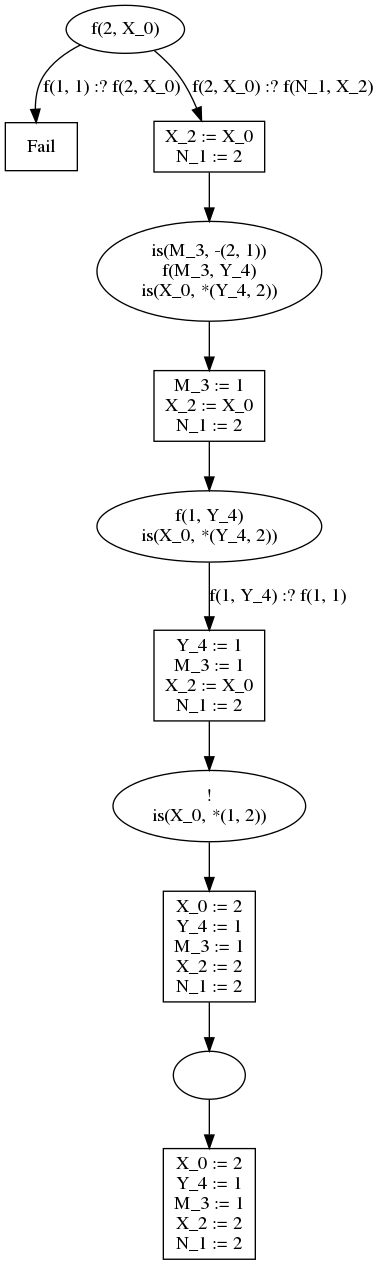
\includegraphics[width=0.4\textwidth]{../fact.png}
		\caption{Дерево поиска решения для факториала}
		\label{uc:1}}
\end{figure}
 

%\include{5-expiremental}

\backmatter %% Здесь заканчивается нумерованная часть документа и начинаются ссылки и

\chapter{Заключение}
В результате проделанной работы, был разработан синтаксический анализатор языка Пролог, реализованы алгоритм унификации и частично алгоритм поиска решений.
Алгоритм поиска решений работает корректно, только в случае если отсечения нет, или оно расположено в конце тела правила.
            %% заключение

%\include{60-conclusion}


\begin{thebibliography}{9}
	 
	 \bibitem{haskell} Изучаем Haskell /Мена А.С. -- Санкт-Петербург: Питер, 2015. -- 464 pp.
	 
	 \bibitem{haskell} Основы программирования на языке Пролог. Курс лекций /Павел Шрайнер -- Интернет-университет информационных технологий, 2005. -- 176 pp.
	 
	 \bibitem{s} Создаём парсер для ini-файлов на Haskell
	  [Электронный ресурс]. Режим https://habr.com/post/50337/, свободный.
	 
	 \bibitem{s} ISO Prolog: A Summary of the Draft Proposed Standard [Электронный ресурс]. Режим доступа: http://fsl.cs.illinois.edu/images/9/9c/PrologStandard.pdf, свободный.
	 
	 \bibitem{s} parsec: Monadic parser combinators [Электронный ресурс]. Режим доступа: http://hackage.haskell.org/package/parsec, свободный.
	 
	 
\end{thebibliography}

%\appendix   % Тут идут приложения

%\include{90-appendix1}
%\include{91-appendix2}

\end{document}

%%% Local Variables:
%%% mode: latex
%%% TeX-master: t
%%% End:
